% (c) 2020 Stefan Antonowicz
% Based off of tex found at https://github.com/ludus-leonis/nipajin
% This file is released under Creative Commons
% Attribution-NonCommercial-ShareAlike 4.0 International License.
% Please do not apply other licenses one-way.

\renewcommand{\yggResearch}{%
  \mychapter{Research}{research}
}

\renewcommand{\yggResearchText}{%


The oddities below can only be created by using Research.  Research can only be used during a Vacation.  More notes on Research can be found in the Core Rules.  

Research is divided into 3 generic types - Iron, Silver, and Gold - with the following costs:


\mytable{X X X} {
    \thead{Type} & \thead{Research} & \thead{Cost} \\
} {
    Iron & 1 & 100\FE \\
    Silver & 3 & 200\AG \\
    Gold & 5 & 500\AU
}

The "Cost" is a generic amount to reflect the materials needed to manifest the fruits of your Research - special books, alembics, inks, quills, etc.   The amount paid counts towards your XP.

%%%%%%%%%%%%%%%%%%%%%%%%%%%%%%%%%%%%%%%%%%%%
%%% CHYMISTRY
%%%%%%%%%%%%%%%%%%%%%%%%%%%%%%%%%%%%%%%%%%%%



\mysection{Chymistry}{research-chymistry}

Researching the transformation of matter into magic, Chymistry is practiced in Civilization during a Vacation.  Practicing Chymistry requires the Settlement where you're taking the Vacation to have a Library (see the Core Rules).  There are 4 basic kinds of chymicals:

\mylist {
  \item \mybold{Tonics}  are mixtures of booze, narcotics, and other things you probably don't want to know about. They must be drunk
  \item \mybold{Powders} can be drunk (in wine), inhaled, or smoked.  If you blow a powder in some Monster’s face, the Monster has to be able to breathe (so they don't work on undead, for example)
  \item \mybold{Sera} need to be injected via a syringe.  If the recipient is a person, they have to have a vein of some kind.  If the recipient is an object, it has to be something a needle could pierce (like an apple)
  \item \mybold{Ungeants} include oils, salves, lubricants, and pastes - basically anything you rub on things (heh heh).  They're usually super viscous and anyone will know the moment they try to drink it.  You can coat a weapon with an unguent  and "apply" it to a Monster by injuring them with the weapon (1 point of damage or more to Flesh).  If your attack misses the unguent doesn't rub off, but if you hit armor / scales / etc. without piercing Flesh, it does.  Unguents can be rubbed on someone who is who is unconscious or petrified.  Can’t be eaten -  tastes shitty and the person will spit it out.
}


  \begin{center}
  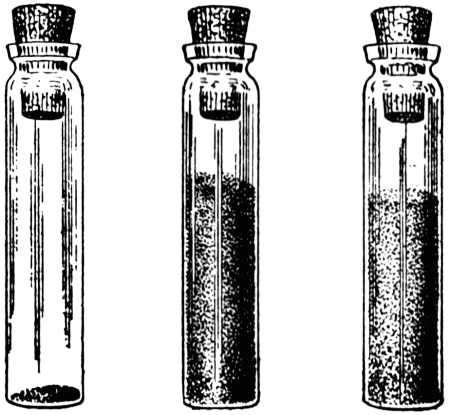
\includegraphics[scale=.5]{Chymistry}
  \end{center}


\mysubsection{Such Mortal Drugs I Have (Toxins)}{research-chymistry-toxins}

You can create a Toxin in the form of a Tonic, Unguent, Sera, or Powder. The efficacy of the potion depends on the type:

  \mytable{X c X} {
    \thead{Type} & \thead{Damage \& Duration} & \thead{Saves}  \\
  } {
     Iron & d4 & 1  \\
     Silver & d8 & 2  \\
     Gold & d12 & 3  \\
  }

  The die type is the amount of damage over a number of minutes (not Minutes, which is its own unit of time), rolled separately. Thus, a Silver Toxin would deal d8 damage for d8 minutes (the Arbiter is encouraged to roll the duration in secret). Damage hits Grit first (as it wears away your will to live), then Flesh.  You cannot heal Grit while under the effects of a Toxin.  The victim of these Toxins \mybold{always} gets a Save (though see below). 

  When Saving against one of these Toxins, the victim can make a Save every minute \myital{before} they are affected by the damage.  If they make the Save, they do not take damage that minute, BUT the Save does not necessarily end the effect of the Toxin.  In order to shake off the effect of the Toxin, the victim must make a number of rolls equal to the Toxin's Duration.  The Saves do not have to be consecutive. 

  When using a Toxin, you must make a \RS : \DEX or risk poisoning yourself unless you have the Knave Virtue \mybold{Poisonous} (see Core Rules)


  \example {
Andre Preneur (Grit 7, Flesh 6) drinks a Silver Toxin hidden in a glass of wine.  The Arbiter rolls the duration (d8) and gets a 7; the effect will last 7 minutes. The Arbiter starts a timer.  Andre rolls a Save and fails - the Arbiter rolls a d8 and gets a 6.  Andre applies the damage (1 Grit, 6 Flesh).  Another minute passes, Andre rolls a Save and makes it. At the 3rd minute, Andre rolls his Save and fails.  The Arbiter rolls 8 damage.  Andre is now Dying.  He will need to roll his \DEATH every time he takes damage from the Toxin for the next 4 minutes, unless he makes 2 more Saves
  }

  \mysubsection{Potent Waters (Acids)}{research-chymistry-acids}

  In addition to Toxins, you can create various kinds of acids.  Acids are always treated as if they were unguents (though they are on the liquid side), and will dissolve flesh, stone, wood, or metal.  They are often used for etching, ruining locks, and pouring on people you hate.  Like Toxins, you must make a \RS : \DEX when using acids or risk pouring them on yourself.

  \mytable{X c} {
    \thead{Type} & \thead{\# Effects}  \\
  } {
     Iron & 1  \\
     Silver & 2  \\
     Gold & 3 \\
  }

  Iron acids allow you to pick one of the results below; Silver acids allow you to pick 2; and Gold acids allow you to take all 3.

  \mybullet {
    \item if the acid hits Flesh, deals d4 damage for d4 Minutes. If it hits Armor, removes 1 \UD every Minute. 
    \item the acid can melt an area 100cm cubed of wood, metal, or stone
    \item the acid will create an acrid plume of smoke that causes coughing and choking for Minutes to everything Nearby (-2 to \RO and \RB attempts)
  }

  You can sunder your Shield to negate the effect of acids thrown on you.  

  \cbreak

  \mysubsection{Tonics}{research-chymistry-tonics}

  \CHYMISTRY[
    Name=Chyme's Nerve Tonic,
    Link=chymistry-chymes-nerve-tonic,
    Cost=Iron (1),
    Duration=until Bivouac,
    Toxin=No,
    Narcotic=\MAX 1
  ]

  You make all of your \RO and \RB checks at +4, but you can never take a Breather - you're far too restless.  

\CHYMISTRY[
  Name=Cuckhold's Courage,
  Link=chymistry-cuckhold-courage,
  Cost=Iron (1),
  Duration=0,
  Toxin=No,
  Narcotic=\MAX 3 
]

Drinking Cuckhold's Courage restores Grit when imbibed during a Breather.  For every bottle of Cuckhold's Courage drunk, the drinker's Grit is healed or increased (even above \MAX !) by 4.  It cannot heal Flesh (only Grit).  Narcotic



\CHYMISTRY[
  Name=Fulcanelli's Clarifying Elixir,
  Link=chymistry-fulcanelli-clarifying-elixir,
  Cost=Silver (3),
  Duration=until Bivouac/0,
  Toxin=No,
  Narcotic=No 
]


Renders you almost immune to any spells or effects from the Mind paradigm.  If you wouldn't normally get a Save against the effect, you now do.  If you \mybold{do} get a Save against the effect, the Save is at +4.  If taken while under the effect of a Mind spell, immediately gives the imbiber a Save as above and ends its Duration.  Can be used to break the effects of the Philter of von Fuchs (it is rumored that Fulcanelli was under the sway of von Fuchs)

\CHYMISTRY[
  Name=Liebnitz Purgation,
  Link=chymistry-liebnitz-purgation,
  Cost=Silver (3),
  Duration=0 ,
  Toxin=No,
  Narcotic=No 
]

If imbibed while under the effects of an ingested Toxin (Tonic, drunk Powder, or Brew) the poison will be immediately vomited forth intact and will cease to affect the victim.  

\CHYMISTRY[
  Name=Philter of von Fuchs,
  Link=chymistry-philter-von-Fuchs,
  Cost=See Below,
  Duration=See Below,
  Toxin=Yes,
  Narcotic=No 
]

When imbibed, the drinker will fall under the sway of whoever gave them the tonic.  Treat as a \mylink{Charm}{wizardry-charm} spell.  Save Negates.  The duration depends on the amount of Research used:  Iron (1), Days; Silver (3), Weeks; Gold (5), Months.  Can be broken by spells, rituals, etc. that relieve effects of the Mind.

  \begin{center}
  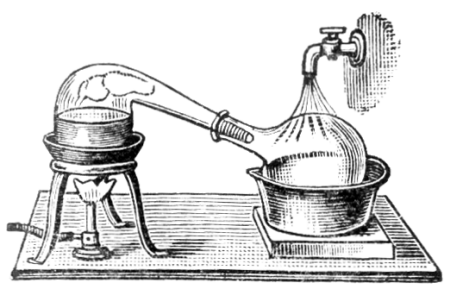
\includegraphics[scale=.5]{Chymistry_2}
  \end{center}


  \mysubsection{Powders}{research-chymistry-powders}

  \CHYMISTRY[
    Name=Dastin's Basic Talc,
    Link=chymistry-dastins-basic-talc,
    Cost=Iron (1),
    Duration=0 ,
    Toxin=No,
    Narcotic=No 
  ]


  Sprinkling this powder on something covered in acid immediately neutralizes the acid (damage, etc).


  \CHYMISTRY[
    Name=Mermaid's Kiss,
    Link=chymistry-mermaids-kiss,
    Cost=Silver (3),
    Duration=0 ,
    Toxin=Yes,
    Narcotic=No 
  ]


  The imbiber stops breathing for Hours.  They can feign death or travel underwater, are not affected by inhaled powders or gases, and are unable to speak or cast spells.  Unwilling victims get a Save (as if this were a Toxin)



  \CHYMISTRY[
    Name=Powdered Bezoar,
    Link=chymistry-powdered-bezoar,
    Cost=Iron (1),
    Duration=0 ,
    Toxin=No,
    Narcotic=No 
  ]


  When sprinkled on a food or into a beverage, has a 5-in-6 chance of neutralizing any Toxin contained inside.  The roll is made in secret by the Arbiter.


  \CHYMISTRY[
    Name=Woundseal,
    Link=chymistry-woundseal,
    Cost=Iron (1),
    Duration=0 ,
    Toxin=No,
    Narcotic=No 
  ]


  Sprinkling this powder on a wound stops all effects of Bleeding, like the Leechcraft skill \mylink{Staunch}{leechcraft-staunch}



  \mysubsection{Ungeants}{research-chymistry-ungeants}
  \CHYMISTRY[
    Name=Boyle's Sharpening Paste,
    Link=chymistry-boyles-sharpening-paste,
    Cost=Iron (1),
    Duration=0 ,
    Toxin=No,
    Narcotic=No 
  ]
  When rubbed on the blade of a stabbing or cutting weapon, the weapon deals +d12 the next time damage is rolled.  The oil rubs off after the strike.


  \CHYMISTRY[
    Name=Brahe's Efficacious Sealant,
    Link=chymistry-brahes-efficacious-sealant,
    Cost=Gold (5),
    Duration=0 ,
    Toxin=No,
    Narcotic=No 
  ]
  Fast-drying paste. Capable of bonding stone, glass, wood, or metal (but not flesh). Lasts forever.  Can cover an area roughly 10cm square.


  \CHYMISTRY[
    Name=Faivre's Aqua Grease,
    Link=chymistry-faivres-aqua-grease,
    Cost=Iron (1),
    Duration=0 ,
    Toxin=No,
    Narcotic=No 
  ]
  A pale grease that can be rubbed over any equipment to completely protect it against damage from water exposure

  \CHYMISTRY[
    Name=Tesla's Silver Wash,
    Link=chymistry-teslas-silver-wash,
    Cost=Silver (3),
    Duration=0 ,
    Toxin=No,
    Narcotic=No 
  ]
  When applied to a 1-handed weapon, the weapon becomes permanently imbued with silver.  Requires an ingot of silver.

  \CHYMISTRY[
    Name=Wei Boyang's Alkahest,
    Link=chymistry-wei-boyangs-alkahest,
    Cost=Gold (5),
    Duration=0 ,
    Toxin=No,
    Narcotic=No 
  ]

  This oil will dissolve any adhesive (including Brahe's Efficacious Sealant).  Can cover an area roughly 10cm square.


\mysubsection{Sera}{research-chymistry-sera}

  \CHYMISTRY[
    Name=Al-Farabi's Calming Injection,
    Link=chymistry-al-farabis-calming-injection,
    Cost=Gold (5),
    Duration=0 ,
    Toxin=Yes,
    Narcotic=No 
  ]

  The injected creature ceases immediately to be Enraged, Shaken, Frenzied, or Disgusted.  If the creature is Zoological, they become passive and docile.  Creatures under the effect of the Calming Injection cannot attack unless they are attacked first.  Lasts for Hours. Unwilling creatures get a Save to negate.

  \CHYMISTRY[
    Name=Davy's Soothing Anesthetic,
    Link=chymistry-davys-soothing-anesthetic,
    Cost=Silver (3),
    Duration=0 ,
    Toxin=Yes,
    Narcotic=No 
  ]

  The injected creature feels any pain as pleasure for Hours.  Often surreptitiously given to those undergoing torture, or going under the knife for surgery.  Attacks against the recipient ignore Grit as the mind loses the cues to shift away from painful events.  


  \CHYMISTRY[
    Name=Grimm's Stupurous Preparation,
    Link=chymistry-grimms-stupurous-preparation,
    Cost=Gold (5),
    Duration=0 ,
    Toxin=Yes,
    Narcotic=No 
  ]


  An injected creature immediately falls into a slumber in all ways like \mylink{Sleep}{wizardry-sleep} (can't be awakened except by a slap, doesn't effect a creature of greater than 4 \HD) unless they Save

  If the sera is injected into solid food of some sort (like an apple), any creature ingesting the food falls into a deep slumber and cannot be awakened except by a Mystic feeding the curse to a 3+ Cunning \mylink{Hekaphage}{occultism-hekaphage}. While asleep the creature is in a state of suspended animation - they do not age, and do not need to eat or drink - but they can still be killed in the normal means (dagger through the heart, etc).  Putting a creature into suspended animation will stop the effects of progressing disease and toxins.  Unwilling creatures get a Save. 

  \CHYMISTRY[
    Name=Wordwarp,
    Link=chymistry-wordwarp,
    Cost=Gold (5),
    Duration=0 ,
    Toxin=Yes,
    Narcotic=No 
  ]

  An oil that causes a form of dyslexia.  If the victim fails a Save, they are unable to read written words for Hours.  Often used on spell casters and scribes.


\newpage

%%%%%%%%%%%%%%%%%%%%%%%%%%%%%%%%%%%%%%%%%%%%
%%% INSCRIPTION
%%%%%%%%%%%%%%%%%%%%%%%%%%%%%%%%%%%%%%%%%%%%



\mysection{Inscription}{research-inscription}

Inscription is the catch-all for mystical control over the written words, incantations, symbols, and engravings that allow Philosophers to capture and control Arcana.  Practicing Inscription requires the Settlement where you're taking the Vacation to have a Library (see the Core Rules). Inscription is generally divided into 4 groups:

\mybullet{
  \item \mylink{Transcription}{research-inscription-transcription}: Writing magical texts to Fetishes and Grimoires
  \item \mylink{Tattoo}{research-inscription-tattoo}: Branding and marking the flesh of living things with magical symbols
  \item \mylink{Sigils}{research-inscription-sigils}: Etching and scribing runes and powerful names 
}

  \begin{center}
  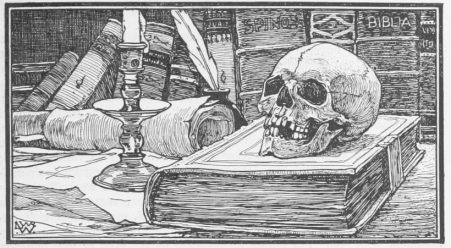
\includegraphics[scale=.5]{Inscription_1}
  \end{center}



\mysubsection{Transcription}{research-inscription-transcription}

Transcription is used to: 
\mybullet {
  \item prepare a new Grimoire so that it "belongs" to you; or
  \item defuse a Grimoire you've stolen from another wizard; or
  \item scribe a spell from a Fetish into a Grimoire; or
  \item scribe a spell from your Grimoire to a Fetish
}

\myhighlight{Preparing Grimoires}{inscription-preparing-grimoires}

By purchasing a blank Grimoire and placing one or more \mylink{Wizard Sigils}{research-sigil-wizard} on it, the Grimoire becomes yours and can now have spells written into it with Scribing (see below).  It is also trapped and needs to be defused in order to be read by another.   You can place as many Wizard Sigils on your Grimoire(s) as you can afford, making them harder to defuse - but you must create all of the Wizard Sigils at once.

\myhighlight{Defusing Grimoires}{inscription-defusing-grimoires}

In order to read another's Grimoire, you must defuse the traps inside.  You must spend a Research for every Wizard Sigil on the Grimoire.  You can read a Grimoire even if it's trapped, but that sets the traps off (this removes the Sigil(s), however).  Roll on \mylink{Grimoire Traps}{grimoire-traps} once for each Sigil.

\myhighlight{Scribing: Fetish to Grimoire}{inscription-scribing-fetish-to-grimoire}

You can write a spell from a Fetish (including a Philosopher's skull) to your Grimoire.  Doing so erases the spell from the Fetish or skull no matter how many \UD it had remaining.  Scribing a spell into your Grimoire is an Iron craft (1 Research; 100\FE)

\myhighlight{Scribing: Grimoire to Fetish}{inscription-scribing-grimoire-to-fetish}

You create a Fetish containing a spell.  The Fetish can be a papyrus, set of mouse skulls, handle of an axe, roll of snakeskin, etc. etc.  The item can't be living (that would be a Tattoo) but can be anything you desire.  A Fetish can only have a single spell on it.  All Fetishes have a \UD of d4 - when the \UD is exhausted, the magical words disappear from the Fetish. 

You may cast the spell inscribed on the Fetish with any number of Blood you choose, OR you may forgo the Blood die and roll a single d6 for the effect.  You still roll the \UD for the Fetish either way.

Creating a Fetish is an Iron craft (1 Research; 100\FE)


\mysubsection{Tattoo}{research-inscription-tattoo}

Tattoos can be inscribed on the body as specified below.  Creating a tattoo is a Silver craft (3 Research; 300\AG).  You can't move a tattoo from yourself to someone else - the tattoo stays with the person.  The tattoos below are the most common, but work out with the Arbiter if you want something more esoteric ...

\myhighlight{Dagger (Limb)}{sorcerer-tattoo-dagger}

Touching the dagger immediately brings it into your hand.  Place the dagger back on the limb returns it to being a tattoo.  The dagger is normal in all ways.

\myhighlight{Torch (Limb)}{sorcerer-tattoo-torch}

As dagger above.  The torch never goes out.

  \begin{center}
  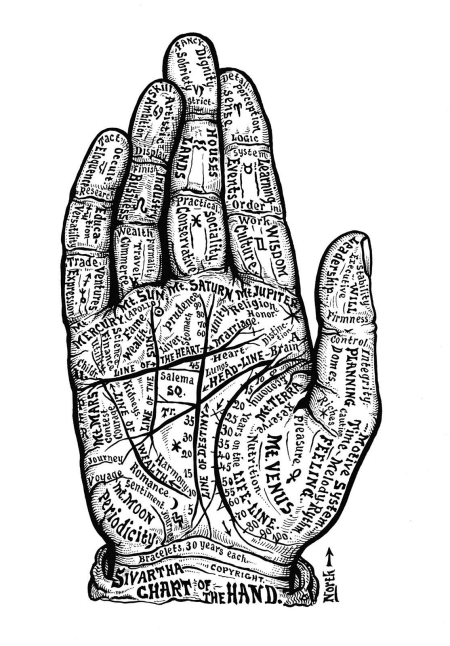
\includegraphics[scale=.5]{Tattoo}
  \end{center}


\myhighlight{Compass (Limb)}{sorcerer-tattoo-compass}

Always points towards true north.  

\myhighlight{Quill and Scroll (Back)}{sorcerer-tattoo-quill-scroll}

The quill can be removed as the Dagger, above - and given to someone else.  Anything that the other person writes with the quill will appear on the scroll tatooed on your Flesh ... painfully.  The writing disappears in Minutes.

\myhighlight{Eye (Palm)}{sorcerer-tattoo-eye}

The tattooed can see through the eye as if it were one of their normal eyes

\myhighlight{Rope (Neck, Arms, Legs, Torso}{sorcerer-tattoo-rope}

As Dagger above, 25m of rope. Needs to be completely rewound around the person to return to being a tattoo.


\myhighlight{Mermaid (chest or neck)}{sorcerer-tattoo-mermaid}

The Philosopher inscribes this tattoo on you and a \mylink{Wizard Sigil}{research-sigil-wizard} on a different object (usually a ship in a bottle or a scrimshawed whale bone).  You do not need to breathe to stay alive - you draw breath instead from the area immediately around the object.  This means that if the object is immersed in water, or sealed in an airtight container, you will suffocate.

\mysubsection{Sigils}{research-inscription-sigils}

Sigils are runes etched into surfaces.  Sigils glow slightly and exude arcane mystery, and are really obvious to everyone Nearby - but what the rune does is only interpretable with a successful Skill:Lore check.  The creation of a new Sigil causes any previous Sigils of the same type created by the Philosopher to vanish.

A Sigil you encounter may be lifeless.  Sigils remain even after their magic is exhausted; only the Philosopher who created the Sigil can erase it from existence by placing a finger on it and reading its name aloud (note: the finger does not need to be attached to the hand, and the finger doesn't have to have flesh on it).  The power of the Sigil depends on the type created.

Unless otherwise specified, a Sigil can only be placed on something that is generally immobile and not alive - a door, a wall, the floor, a statue, etc.  Philosophers are immune to their own Sigil's effects where appropriate.  Sigils are permanent unless noted (even if they are lifeless).

\large{\mybold{Iron Sigils}}\normalsize

\example{
   1 Research \& 100\FE
}


\myanchor{\mybold{Chaining Sigil}}{research-sigil-chaining}  

A Chaining Sigil can be scribed and "married" to another Sigil.  The Chaining Sigil must be created at the same time as its partner Sigil.  If a Chaining Sigil is erased by the Sorcerer who inscribed it, the Sigil it is partnered with will immediately manifest.  Chaining Sigils are permanent until dispelled.

\myanchor{\mybold{Talking Sigil}}{research-sigil-talking} 

When anyone comes Close to an object with a Talking Sigil on it, it will yell out a number of words at ear-splitting volume.  It will repeat these words a number of times, depending on the Research spent.

Each additional word/time you want the Talking Sigil to speak, you must spend an additional +1 Research/+100\FE.


\myanchor{\mybold{ Warding Sigil}}{research-sigil-warding}

This glyph can only be placed on something that is closed : a book, a lock, a chest but not a sword in a scabbard or someone's mouth (Arbiter's discretion).  If the warded item is opened, the Sigil immediately becomes lifeless.

When anyone comes Close to an item with a Warding Sigil on it, they must Save or move somewhere Nearby, back the way they came.  

For each 1 Research/100\FE you spend past the initial cost, the Warding Sigil affects a -2 modifier on the Save.


\myanchor{\mybold{Wizard Sigil}}{research-sigil-wizard}

The most basic Sigil, essentially just the Sorcerer's name - but necessary to allow a weapon, object, or person to be a receptacle for magic.  The inscriber of the Wizard Sigil can only be determined with a successful Skill:Lore role.


\large{\mybold{Silver Sigils}}\normalsize


\example{
   3 Research \& 300\AG
}


\myanchor{\mybold{Cursing Sigil}}{research-sigil-cursing}

This Sigil can only be created with the help of a Mystic, who must use Cunning to create the \mylink{Malison}{occultism-malison} that resides in the Sigil.  When anyone comes Close to an object with the Sigil on it, they must Save vs. Hexes or fall victim to the curse. If there is more than 1 target, they should hold a Luck contest.

For each 1 Research/100\AG you spend past the initial cost, the Cursing Sigil affects a -2 modifier on the Save.


\myanchor{\mybold{Elemental Sigil}}{research-sigil-elemental}

When anyone comes Close to an object with an Elemental Sigil on it, they are dealt 5 elemental damage.  The inscriber chooses the elemental type (lightning, fire, etc).  Save for half damage.

For each 1 Research/100\AG you spend past the initial cost, the Elemental Sigil deals +2 damage


\myanchor{\mybold{ Petrifying Sigil}}{research-sigil-petrifying}

When anyone comes Close to a Petrifying Sigil, they must Save or become Paralyzed.  The duration of the paralysis lasts until the Sigil is erased. You age while you are paralyzed.

\myanchor{\mybold{Portal Sigil}}{research-sigil-portal}

These must be placed on doors, gates, or entrances.  A Portal Sigil is placed on the threshold or top of one doorway and a Wizard Sigil is placed on another; the two doors are connected as if they are the same door.  Someone stepping through the Portal Sigil side will exit through the \mylink{Wizard Sigil}{research-sigil-wizard} side (but not vice-versa).  Erasing either Sigil closes the doorway.

\large{\mybold{Gold Sigils}}\normalsize


\example{
   5 Research \& 500\AU
}



\myanchor{\mybold{ Erasing Sigil }}{research-sigil-erasing}

When anyone comes close to an Erasing Sigil, they must Save or suffer one of the effects below (roll a d6):

\mynumlist {
  \item Erases the spells etched in a Sorcerer's mind
  \item Erases everything in a person's backpack
  \item Erases a person's armor and weapons (magic items get an additional Save)
  \item Erases all coins a person is carrying
  \item Erases a person's Grit, bringing it to zero
  \item Erases a person's Flesh and they are Dying
}

For each 1 Research/100\AU you spend past the initial cost, the Erasing Sigil affects a -2 modifier on the Save.

\cbreak

\myanchor{\mybold{Remembrance Sigil}}{research-sigil-remembrance}

This Sigil can only be created with the help of a Spriggan, who will place one of the \mylink{Obliterated}{forgotten-obliterated} inside of the Sigil.  The maximum \HD of the creature starts at 2; for each 1 Research/100\AU you spend past the initial cost, this maximum is increased by +1.

Anyone other than the Sorcerer or Spriggan who comes Close to the Remembrance Sigil will cause the Obliterated to come forth - very pissed off - and immediately attack.  If the Obliterated is slain, the Sigil will become lifeless.

\cbreak

\myanchor{\mybold{Revisitation Sigil}}{research-sigil-revisitation}

The Revisitation Sigil is scribed as normal (usually on a floor in the Sorcerer's laboratory) and a \mylink{Chaining Sigil}{research-sigil-chaining} is placed on another portable item.  When the Chaining Sigil is erased, the Sorcerer is transported to the location of the Revisitation Sigil.  

For each 1 Research/100\AU you spend past the initial cost, you can bring 1 other Ally with you.


\newpage
%%%%%%%%%%%%%%%%%%%%%%%%%%%%%%%%%%%%%%%%%%%%
%%% MEDICINALS
%%%%%%%%%%%%%%%%%%%%%%%%%%%%%%%%%%%%%%%%%%%%

\mysection{Medicinals}{research-medicinals}

Medicinals allow a Philosopher to heal the more permanent ailments that might be afflicting the other members of the Band.   To practice your craft, the Settlement where you're taking the Vacation must have a Sanitarium and/or Library present (see the Core Rules).  Medicinals require no coin, but you can make a donation to the Sanitarium or Library if you'd like (up 200 coins of the appropriate type per Research spent) in order to convert coin to XP.

\mysubsection{Cure Disease}{research-medicinals-cure-disease}

\example{
   2 Research per Disease
}

You can cure any disease currently infecting your Ally.  Each disease requires 2 Research.

  \begin{center}
  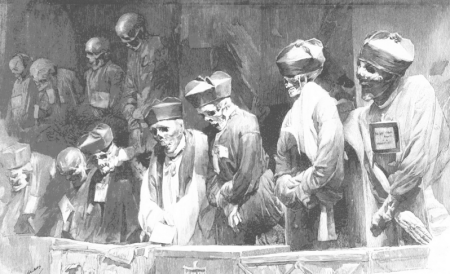
\includegraphics[scale=.5]{Medicinals}
  \end{center}

\cbreak

\mysubsection{Rehab}{research-medicinals-rehab}

\example{
   6 - (\MAX Overdose) Research
}


You can cure someone's addiction to Narcotics.  The cost is a number of Research equal to 6 minus the \MAX Overdose rating of the narcotic in question (for example, Pipeweed has a \MAX Overdose of 4, so it would require 2 Research; Yellow Opium has a \MAX Overdose of 1, so it would require 5 Research).  The recovering addict will have the permanent effect listed under Recovery (see the Core Rules).

\mysubsection{Wounds}{research-medicinals-wounds}

\example{
   2 Research per Wound
}


Through your gentle ministrations over the course of a Vacation, you heal a patient's Beating, Madness, or Life Drain.  The cost is 2 Research per Wound mended.




}%end
